\documentclass[twoside]{book}

% Packages required by doxygen
\usepackage{fixltx2e}
\usepackage{calc}
\usepackage{doxygen}
\usepackage[export]{adjustbox} % also loads graphicx
\usepackage{graphicx}
\usepackage[utf8]{inputenc}
\usepackage{makeidx}
\usepackage{multicol}
\usepackage{multirow}
\PassOptionsToPackage{warn}{textcomp}
\usepackage{textcomp}
\usepackage[nointegrals]{wasysym}
\usepackage[table]{xcolor}

% Font selection
\usepackage[T1]{fontenc}
\usepackage[scaled=.90]{helvet}
\usepackage{courier}
\usepackage{amssymb}
\usepackage{sectsty}
\renewcommand{\familydefault}{\sfdefault}
\allsectionsfont{%
  \fontseries{bc}\selectfont%
  \color{darkgray}%
}
\renewcommand{\DoxyLabelFont}{%
  \fontseries{bc}\selectfont%
  \color{darkgray}%
}
\newcommand{\+}{\discretionary{\mbox{\scriptsize$\hookleftarrow$}}{}{}}

% Page & text layout
\usepackage{geometry}
\geometry{%
  a4paper,%
  top=2.5cm,%
  bottom=2.5cm,%
  left=2.5cm,%
  right=2.5cm%
}
\tolerance=750
\hfuzz=15pt
\hbadness=750
\setlength{\emergencystretch}{15pt}
\setlength{\parindent}{0cm}
\setlength{\parskip}{3ex plus 2ex minus 2ex}
\makeatletter
\renewcommand{\paragraph}{%
  \@startsection{paragraph}{4}{0ex}{-1.0ex}{1.0ex}{%
    \normalfont\normalsize\bfseries\SS@parafont%
  }%
}
\renewcommand{\subparagraph}{%
  \@startsection{subparagraph}{5}{0ex}{-1.0ex}{1.0ex}{%
    \normalfont\normalsize\bfseries\SS@subparafont%
  }%
}
\makeatother

% Headers & footers
\usepackage{fancyhdr}
\pagestyle{fancyplain}
\fancyhead[LE]{\fancyplain{}{\bfseries\thepage}}
\fancyhead[CE]{\fancyplain{}{}}
\fancyhead[RE]{\fancyplain{}{\bfseries\leftmark}}
\fancyhead[LO]{\fancyplain{}{\bfseries\rightmark}}
\fancyhead[CO]{\fancyplain{}{}}
\fancyhead[RO]{\fancyplain{}{\bfseries\thepage}}
\fancyfoot[LE]{\fancyplain{}{}}
\fancyfoot[CE]{\fancyplain{}{}}
\fancyfoot[RE]{\fancyplain{}{\bfseries\scriptsize Generated by Doxygen }}
\fancyfoot[LO]{\fancyplain{}{\bfseries\scriptsize Generated by Doxygen }}
\fancyfoot[CO]{\fancyplain{}{}}
\fancyfoot[RO]{\fancyplain{}{}}
\renewcommand{\footrulewidth}{0.4pt}
\renewcommand{\chaptermark}[1]{%
  \markboth{#1}{}%
}
\renewcommand{\sectionmark}[1]{%
  \markright{\thesection\ #1}%
}

% Indices & bibliography
\usepackage{natbib}
\usepackage[titles]{tocloft}
\setcounter{tocdepth}{3}
\setcounter{secnumdepth}{5}
\makeindex

% Hyperlinks (required, but should be loaded last)
\usepackage{ifpdf}
\ifpdf
  \usepackage[pdftex,pagebackref=true]{hyperref}
\else
  \usepackage[ps2pdf,pagebackref=true]{hyperref}
\fi
\hypersetup{%
  colorlinks=true,%
  linkcolor=blue,%
  citecolor=blue,%
  unicode%
}

% Custom commands
\newcommand{\clearemptydoublepage}{%
  \newpage{\pagestyle{empty}\cleardoublepage}%
}

\usepackage{caption}
\captionsetup{labelsep=space,justification=centering,font={bf},singlelinecheck=off,skip=4pt,position=top}

%===== C O N T E N T S =====

\begin{document}

% Titlepage & ToC
\hypersetup{pageanchor=false,
             bookmarksnumbered=true,
             pdfencoding=unicode
            }
\pagenumbering{roman}
\begin{titlepage}
\vspace*{7cm}
\begin{center}%
{\Large My Project }\\
\vspace*{1cm}
{\large Generated by Doxygen 1.8.11}\\
\end{center}
\end{titlepage}
\clearemptydoublepage
\tableofcontents
\clearemptydoublepage
\pagenumbering{arabic}
\hypersetup{pageanchor=true}

%--- Begin generated contents ---
\chapter{Hierarchical Index}
\section{Class Hierarchy}
This inheritance list is sorted roughly, but not completely, alphabetically\+:\begin{DoxyCompactList}
\item \contentsline{section}{Fruit}{\pageref{classFruit}}{}
\begin{DoxyCompactList}
\item \contentsline{section}{Apple}{\pageref{classApple}}{}
\item \contentsline{section}{Grape}{\pageref{classGrape}}{}
\item \contentsline{section}{Orange}{\pageref{classOrange}}{}
\end{DoxyCompactList}
\item \contentsline{section}{List}{\pageref{classList}}{}
\item \contentsline{section}{List\+:\+:Node}{\pageref{structList_1_1Node}}{}
\end{DoxyCompactList}

\chapter{Class Index}
\section{Class List}
Here are the classes, structs, unions and interfaces with brief descriptions\+:\begin{DoxyCompactList}
\item\contentsline{section}{\hyperlink{structnode}{node} }{\pageref{structnode}}{}
\item\contentsline{section}{\hyperlink{structnode1}{node1} }{\pageref{structnode1}}{}
\item\contentsline{section}{\hyperlink{structnode__info}{node\+\_\+info} }{\pageref{structnode__info}}{}
\end{DoxyCompactList}

\chapter{File Index}
\section{File List}
Here is a list of all files with brief descriptions\+:\begin{DoxyCompactList}
\item\contentsline{section}{\hyperlink{Lab1_8c}{Lab1.\+c} }{\pageref{Lab1_8c}}{}
\end{DoxyCompactList}

\chapter{Class Documentation}
\hypertarget{classDeluxePizza}{}\section{Deluxe\+Pizza Class Reference}
\label{classDeluxePizza}\index{Deluxe\+Pizza@{Deluxe\+Pizza}}


Inheritance diagram for Deluxe\+Pizza\+:
\nopagebreak
\begin{figure}[H]
\begin{center}
\leavevmode
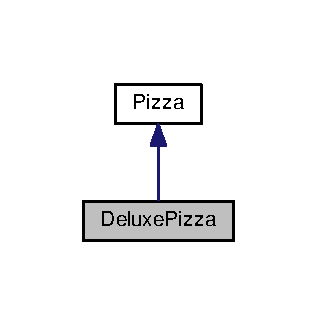
\includegraphics[width=152pt]{classDeluxePizza__inherit__graph}
\end{center}
\end{figure}


Collaboration diagram for Deluxe\+Pizza\+:
\nopagebreak
\begin{figure}[H]
\begin{center}
\leavevmode
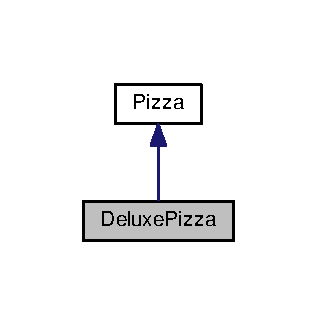
\includegraphics[width=152pt]{classDeluxePizza__coll__graph}
\end{center}
\end{figure}
\subsection*{Public Member Functions}
\begin{DoxyCompactItemize}
\item 
virtual int \hyperlink{classDeluxePizza_af66f2ac20b82113fc5507a83b63f713c}{get\+Price} () const 
\item 
virtual \hyperlink{classDeluxePizza_a010c07d4617e9fc49d35108057cf6678}{$\sim$\+Deluxe\+Pizza} ()
\end{DoxyCompactItemize}


\subsection{Constructor \& Destructor Documentation}
\index{Deluxe\+Pizza@{Deluxe\+Pizza}!````~Deluxe\+Pizza@{$\sim$\+Deluxe\+Pizza}}
\index{````~Deluxe\+Pizza@{$\sim$\+Deluxe\+Pizza}!Deluxe\+Pizza@{Deluxe\+Pizza}}
\subsubsection[{\texorpdfstring{$\sim$\+Deluxe\+Pizza()}{~DeluxePizza()}}]{\setlength{\rightskip}{0pt plus 5cm}virtual Deluxe\+Pizza\+::$\sim$\+Deluxe\+Pizza (
\begin{DoxyParamCaption}
{}
\end{DoxyParamCaption}
)\hspace{0.3cm}{\ttfamily [inline]}, {\ttfamily [virtual]}}\hypertarget{classDeluxePizza_a010c07d4617e9fc49d35108057cf6678}{}\label{classDeluxePizza_a010c07d4617e9fc49d35108057cf6678}

\begin{DoxyCode}
21 \{\};
\end{DoxyCode}


\subsection{Member Function Documentation}
\index{Deluxe\+Pizza@{Deluxe\+Pizza}!get\+Price@{get\+Price}}
\index{get\+Price@{get\+Price}!Deluxe\+Pizza@{Deluxe\+Pizza}}
\subsubsection[{\texorpdfstring{get\+Price() const }{getPrice() const }}]{\setlength{\rightskip}{0pt plus 5cm}virtual int Deluxe\+Pizza\+::get\+Price (
\begin{DoxyParamCaption}
{}
\end{DoxyParamCaption}
) const\hspace{0.3cm}{\ttfamily [inline]}, {\ttfamily [virtual]}}\hypertarget{classDeluxePizza_af66f2ac20b82113fc5507a83b63f713c}{}\label{classDeluxePizza_af66f2ac20b82113fc5507a83b63f713c}


Implements \hyperlink{classPizza_aa9c7966d23241bfa79efe9f7d9f45408}{Pizza}.


\begin{DoxyCode}
20 \{ \textcolor{keywordflow}{return} 1050; \};
\end{DoxyCode}


The documentation for this class was generated from the following file\+:\begin{DoxyCompactItemize}
\item 
\hyperlink{Factory_8cpp}{Factory.\+cpp}\end{DoxyCompactItemize}

\hypertarget{classHamAndMushroomPizza}{}\section{Ham\+And\+Mushroom\+Pizza Class Reference}
\label{classHamAndMushroomPizza}\index{Ham\+And\+Mushroom\+Pizza@{Ham\+And\+Mushroom\+Pizza}}


Inheritance diagram for Ham\+And\+Mushroom\+Pizza\+:
\nopagebreak
\begin{figure}[H]
\begin{center}
\leavevmode
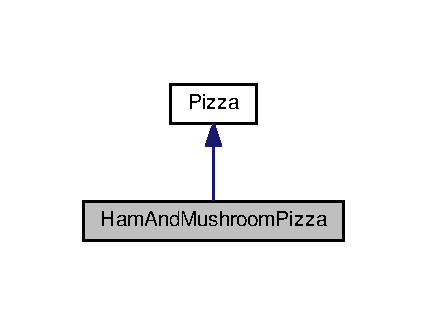
\includegraphics[width=205pt]{classHamAndMushroomPizza__inherit__graph}
\end{center}
\end{figure}


Collaboration diagram for Ham\+And\+Mushroom\+Pizza\+:
\nopagebreak
\begin{figure}[H]
\begin{center}
\leavevmode
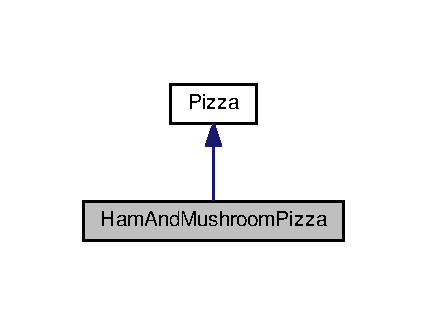
\includegraphics[width=205pt]{classHamAndMushroomPizza__coll__graph}
\end{center}
\end{figure}
\subsection*{Public Member Functions}
\begin{DoxyCompactItemize}
\item 
virtual int \hyperlink{classHamAndMushroomPizza_a90a3473504de97256e1b46d7ab60eebb}{get\+Price} () const 
\item 
virtual \hyperlink{classHamAndMushroomPizza_af7d5144bb5cfcee53599f12118282c93}{$\sim$\+Ham\+And\+Mushroom\+Pizza} ()
\end{DoxyCompactItemize}


\subsection{Constructor \& Destructor Documentation}
\index{Ham\+And\+Mushroom\+Pizza@{Ham\+And\+Mushroom\+Pizza}!````~Ham\+And\+Mushroom\+Pizza@{$\sim$\+Ham\+And\+Mushroom\+Pizza}}
\index{````~Ham\+And\+Mushroom\+Pizza@{$\sim$\+Ham\+And\+Mushroom\+Pizza}!Ham\+And\+Mushroom\+Pizza@{Ham\+And\+Mushroom\+Pizza}}
\subsubsection[{\texorpdfstring{$\sim$\+Ham\+And\+Mushroom\+Pizza()}{~HamAndMushroomPizza()}}]{\setlength{\rightskip}{0pt plus 5cm}virtual Ham\+And\+Mushroom\+Pizza\+::$\sim$\+Ham\+And\+Mushroom\+Pizza (
\begin{DoxyParamCaption}
{}
\end{DoxyParamCaption}
)\hspace{0.3cm}{\ttfamily [inline]}, {\ttfamily [virtual]}}\hypertarget{classHamAndMushroomPizza_af7d5144bb5cfcee53599f12118282c93}{}\label{classHamAndMushroomPizza_af7d5144bb5cfcee53599f12118282c93}

\begin{DoxyCode}
15 \{\};
\end{DoxyCode}


\subsection{Member Function Documentation}
\index{Ham\+And\+Mushroom\+Pizza@{Ham\+And\+Mushroom\+Pizza}!get\+Price@{get\+Price}}
\index{get\+Price@{get\+Price}!Ham\+And\+Mushroom\+Pizza@{Ham\+And\+Mushroom\+Pizza}}
\subsubsection[{\texorpdfstring{get\+Price() const }{getPrice() const }}]{\setlength{\rightskip}{0pt plus 5cm}virtual int Ham\+And\+Mushroom\+Pizza\+::get\+Price (
\begin{DoxyParamCaption}
{}
\end{DoxyParamCaption}
) const\hspace{0.3cm}{\ttfamily [inline]}, {\ttfamily [virtual]}}\hypertarget{classHamAndMushroomPizza_a90a3473504de97256e1b46d7ab60eebb}{}\label{classHamAndMushroomPizza_a90a3473504de97256e1b46d7ab60eebb}


Implements \hyperlink{classPizza_aa9c7966d23241bfa79efe9f7d9f45408}{Pizza}.


\begin{DoxyCode}
14 \{ \textcolor{keywordflow}{return} 850; \};
\end{DoxyCode}


The documentation for this class was generated from the following file\+:\begin{DoxyCompactItemize}
\item 
\hyperlink{Factory_8cpp}{Factory.\+cpp}\end{DoxyCompactItemize}

\hypertarget{classHawaiianPizza}{}\section{Hawaiian\+Pizza Class Reference}
\label{classHawaiianPizza}\index{Hawaiian\+Pizza@{Hawaiian\+Pizza}}


Inheritance diagram for Hawaiian\+Pizza\+:
\nopagebreak
\begin{figure}[H]
\begin{center}
\leavevmode
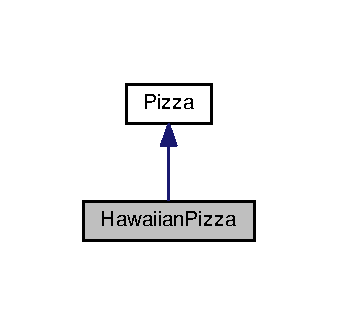
\includegraphics[width=162pt]{classHawaiianPizza__inherit__graph}
\end{center}
\end{figure}


Collaboration diagram for Hawaiian\+Pizza\+:
\nopagebreak
\begin{figure}[H]
\begin{center}
\leavevmode
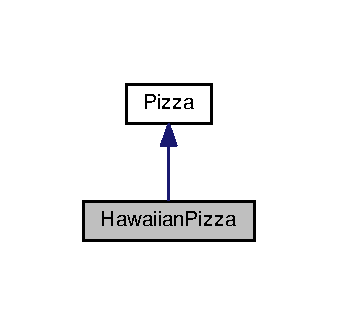
\includegraphics[width=162pt]{classHawaiianPizza__coll__graph}
\end{center}
\end{figure}
\subsection*{Public Member Functions}
\begin{DoxyCompactItemize}
\item 
virtual int \hyperlink{classHawaiianPizza_a04efac994727eeb9d772ce9b6654d4f7}{get\+Price} () const 
\item 
virtual \hyperlink{classHawaiianPizza_a8e5e1cd50df9a52579b3759e59c968dc}{$\sim$\+Hawaiian\+Pizza} ()
\end{DoxyCompactItemize}


\subsection{Constructor \& Destructor Documentation}
\index{Hawaiian\+Pizza@{Hawaiian\+Pizza}!````~Hawaiian\+Pizza@{$\sim$\+Hawaiian\+Pizza}}
\index{````~Hawaiian\+Pizza@{$\sim$\+Hawaiian\+Pizza}!Hawaiian\+Pizza@{Hawaiian\+Pizza}}
\subsubsection[{\texorpdfstring{$\sim$\+Hawaiian\+Pizza()}{~HawaiianPizza()}}]{\setlength{\rightskip}{0pt plus 5cm}virtual Hawaiian\+Pizza\+::$\sim$\+Hawaiian\+Pizza (
\begin{DoxyParamCaption}
{}
\end{DoxyParamCaption}
)\hspace{0.3cm}{\ttfamily [inline]}, {\ttfamily [virtual]}}\hypertarget{classHawaiianPizza_a8e5e1cd50df9a52579b3759e59c968dc}{}\label{classHawaiianPizza_a8e5e1cd50df9a52579b3759e59c968dc}

\begin{DoxyCode}
27 \{\};
\end{DoxyCode}


\subsection{Member Function Documentation}
\index{Hawaiian\+Pizza@{Hawaiian\+Pizza}!get\+Price@{get\+Price}}
\index{get\+Price@{get\+Price}!Hawaiian\+Pizza@{Hawaiian\+Pizza}}
\subsubsection[{\texorpdfstring{get\+Price() const }{getPrice() const }}]{\setlength{\rightskip}{0pt plus 5cm}virtual int Hawaiian\+Pizza\+::get\+Price (
\begin{DoxyParamCaption}
{}
\end{DoxyParamCaption}
) const\hspace{0.3cm}{\ttfamily [inline]}, {\ttfamily [virtual]}}\hypertarget{classHawaiianPizza_a04efac994727eeb9d772ce9b6654d4f7}{}\label{classHawaiianPizza_a04efac994727eeb9d772ce9b6654d4f7}


Implements \hyperlink{classPizza_aa9c7966d23241bfa79efe9f7d9f45408}{Pizza}.


\begin{DoxyCode}
26 \{ \textcolor{keywordflow}{return} 1150; \};
\end{DoxyCode}


The documentation for this class was generated from the following file\+:\begin{DoxyCompactItemize}
\item 
\hyperlink{Factory_8cpp}{Factory.\+cpp}\end{DoxyCompactItemize}

\hypertarget{classPizza}{}\section{Pizza Class Reference}
\label{classPizza}\index{Pizza@{Pizza}}


Inheritance diagram for Pizza\+:
\nopagebreak
\begin{figure}[H]
\begin{center}
\leavevmode
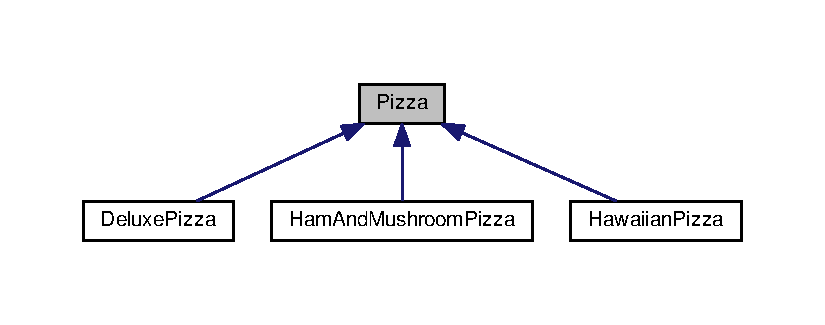
\includegraphics[width=350pt]{classPizza__inherit__graph}
\end{center}
\end{figure}
\subsection*{Public Member Functions}
\begin{DoxyCompactItemize}
\item 
virtual int \hyperlink{classPizza_aa9c7966d23241bfa79efe9f7d9f45408}{get\+Price} () const =0
\item 
virtual \hyperlink{classPizza_a28affbd9b37a895e49aea25360a36a2c}{$\sim$\+Pizza} ()
\end{DoxyCompactItemize}


\subsection{Constructor \& Destructor Documentation}
\index{Pizza@{Pizza}!````~Pizza@{$\sim$\+Pizza}}
\index{````~Pizza@{$\sim$\+Pizza}!Pizza@{Pizza}}
\subsubsection[{\texorpdfstring{$\sim$\+Pizza()}{~Pizza()}}]{\setlength{\rightskip}{0pt plus 5cm}virtual Pizza\+::$\sim$\+Pizza (
\begin{DoxyParamCaption}
{}
\end{DoxyParamCaption}
)\hspace{0.3cm}{\ttfamily [inline]}, {\ttfamily [virtual]}}\hypertarget{classPizza_a28affbd9b37a895e49aea25360a36a2c}{}\label{classPizza_a28affbd9b37a895e49aea25360a36a2c}

\begin{DoxyCode}
9 \{\};  \textcolor{comment}{/* without this, no destructor for derived Pizza's will be called. */}
\end{DoxyCode}


\subsection{Member Function Documentation}
\index{Pizza@{Pizza}!get\+Price@{get\+Price}}
\index{get\+Price@{get\+Price}!Pizza@{Pizza}}
\subsubsection[{\texorpdfstring{get\+Price() const =0}{getPrice() const =0}}]{\setlength{\rightskip}{0pt plus 5cm}virtual int Pizza\+::get\+Price (
\begin{DoxyParamCaption}
{}
\end{DoxyParamCaption}
) const\hspace{0.3cm}{\ttfamily [pure virtual]}}\hypertarget{classPizza_aa9c7966d23241bfa79efe9f7d9f45408}{}\label{classPizza_aa9c7966d23241bfa79efe9f7d9f45408}


Implemented in \hyperlink{classHawaiianPizza_a04efac994727eeb9d772ce9b6654d4f7}{Hawaiian\+Pizza}, \hyperlink{classDeluxePizza_af66f2ac20b82113fc5507a83b63f713c}{Deluxe\+Pizza}, and \hyperlink{classHamAndMushroomPizza_a90a3473504de97256e1b46d7ab60eebb}{Ham\+And\+Mushroom\+Pizza}.



The documentation for this class was generated from the following file\+:\begin{DoxyCompactItemize}
\item 
\hyperlink{Factory_8cpp}{Factory.\+cpp}\end{DoxyCompactItemize}

\hypertarget{classPizzaFactory}{}\section{Pizza\+Factory Class Reference}
\label{classPizzaFactory}\index{Pizza\+Factory@{Pizza\+Factory}}
\subsection*{Public Types}
\begin{DoxyCompactItemize}
\item 
enum \hyperlink{classPizzaFactory_a247cf751b7af4fd338a14303c9e67fe4}{Pizza\+Type} \{ \hyperlink{classPizzaFactory_a247cf751b7af4fd338a14303c9e67fe4ab47db230a75b01a1a531d9374a57dc23}{Ham\+Mushroom}, 
\hyperlink{classPizzaFactory_a247cf751b7af4fd338a14303c9e67fe4ae05ccf2778af31944f7205f550c33e8b}{Deluxe}, 
\hyperlink{classPizzaFactory_a247cf751b7af4fd338a14303c9e67fe4a43552967e3be1afe8d7bf89feb21ba4e}{Hawaiian}
 \}
\end{DoxyCompactItemize}
\subsection*{Static Public Member Functions}
\begin{DoxyCompactItemize}
\item 
static unique\+\_\+ptr$<$ \hyperlink{classPizza}{Pizza} $>$ \hyperlink{classPizzaFactory_ae03b206abf337720e9f019eb735d6131}{create\+Pizza} (\hyperlink{classPizzaFactory_a247cf751b7af4fd338a14303c9e67fe4}{Pizza\+Type} pizza\+Type)
\end{DoxyCompactItemize}


\subsection{Member Enumeration Documentation}
\index{Pizza\+Factory@{Pizza\+Factory}!Pizza\+Type@{Pizza\+Type}}
\index{Pizza\+Type@{Pizza\+Type}!Pizza\+Factory@{Pizza\+Factory}}
\subsubsection[{\texorpdfstring{Pizza\+Type}{PizzaType}}]{\setlength{\rightskip}{0pt plus 5cm}enum {\bf Pizza\+Factory\+::\+Pizza\+Type}}\hypertarget{classPizzaFactory_a247cf751b7af4fd338a14303c9e67fe4}{}\label{classPizzaFactory_a247cf751b7af4fd338a14303c9e67fe4}
\begin{Desc}
\item[Enumerator]\par
\begin{description}
\index{Ham\+Mushroom@{Ham\+Mushroom}!Pizza\+Factory@{Pizza\+Factory}}\index{Pizza\+Factory@{Pizza\+Factory}!Ham\+Mushroom@{Ham\+Mushroom}}\item[{\em 
Ham\+Mushroom\hypertarget{classPizzaFactory_a247cf751b7af4fd338a14303c9e67fe4ab47db230a75b01a1a531d9374a57dc23}{}\label{classPizzaFactory_a247cf751b7af4fd338a14303c9e67fe4ab47db230a75b01a1a531d9374a57dc23}
}]\index{Deluxe@{Deluxe}!Pizza\+Factory@{Pizza\+Factory}}\index{Pizza\+Factory@{Pizza\+Factory}!Deluxe@{Deluxe}}\item[{\em 
Deluxe\hypertarget{classPizzaFactory_a247cf751b7af4fd338a14303c9e67fe4ae05ccf2778af31944f7205f550c33e8b}{}\label{classPizzaFactory_a247cf751b7af4fd338a14303c9e67fe4ae05ccf2778af31944f7205f550c33e8b}
}]\index{Hawaiian@{Hawaiian}!Pizza\+Factory@{Pizza\+Factory}}\index{Pizza\+Factory@{Pizza\+Factory}!Hawaiian@{Hawaiian}}\item[{\em 
Hawaiian\hypertarget{classPizzaFactory_a247cf751b7af4fd338a14303c9e67fe4a43552967e3be1afe8d7bf89feb21ba4e}{}\label{classPizzaFactory_a247cf751b7af4fd338a14303c9e67fe4a43552967e3be1afe8d7bf89feb21ba4e}
}]\end{description}
\end{Desc}

\begin{DoxyCode}
32                    \{
33         \hyperlink{classPizzaFactory_a247cf751b7af4fd338a14303c9e67fe4ab47db230a75b01a1a531d9374a57dc23}{HamMushroom},
34         \hyperlink{classPizzaFactory_a247cf751b7af4fd338a14303c9e67fe4ae05ccf2778af31944f7205f550c33e8b}{Deluxe},
35         \hyperlink{classPizzaFactory_a247cf751b7af4fd338a14303c9e67fe4a43552967e3be1afe8d7bf89feb21ba4e}{Hawaiian}
36     \};
\end{DoxyCode}


\subsection{Member Function Documentation}
\index{Pizza\+Factory@{Pizza\+Factory}!create\+Pizza@{create\+Pizza}}
\index{create\+Pizza@{create\+Pizza}!Pizza\+Factory@{Pizza\+Factory}}
\subsubsection[{\texorpdfstring{create\+Pizza(\+Pizza\+Type pizza\+Type)}{createPizza(PizzaType pizzaType)}}]{\setlength{\rightskip}{0pt plus 5cm}static unique\+\_\+ptr$<${\bf Pizza}$>$ Pizza\+Factory\+::create\+Pizza (
\begin{DoxyParamCaption}
\item[{{\bf Pizza\+Type}}]{pizza\+Type}
\end{DoxyParamCaption}
)\hspace{0.3cm}{\ttfamily [inline]}, {\ttfamily [static]}}\hypertarget{classPizzaFactory_ae03b206abf337720e9f019eb735d6131}{}\label{classPizzaFactory_ae03b206abf337720e9f019eb735d6131}

\begin{DoxyCode}
38                                                               \{
39         \textcolor{keywordflow}{switch} (pizzaType) \{
40         \textcolor{keywordflow}{case} \hyperlink{classPizzaFactory_a247cf751b7af4fd338a14303c9e67fe4ab47db230a75b01a1a531d9374a57dc23}{HamMushroom}: \textcolor{keywordflow}{return} make\_unique<HamAndMushroomPizza>();
41         \textcolor{keywordflow}{case} \hyperlink{classPizzaFactory_a247cf751b7af4fd338a14303c9e67fe4ae05ccf2778af31944f7205f550c33e8b}{Deluxe}:      \textcolor{keywordflow}{return} make\_unique<DeluxePizza>();
42         \textcolor{keywordflow}{case} \hyperlink{classPizzaFactory_a247cf751b7af4fd338a14303c9e67fe4a43552967e3be1afe8d7bf89feb21ba4e}{Hawaiian}:    \textcolor{keywordflow}{return} make\_unique<HawaiianPizza>();
43         \}
44         \textcolor{keywordflow}{throw} \textcolor{stringliteral}{"invalid pizza type."};
45     \}
\end{DoxyCode}


The documentation for this class was generated from the following file\+:\begin{DoxyCompactItemize}
\item 
\hyperlink{Factory_8cpp}{Factory.\+cpp}\end{DoxyCompactItemize}

\chapter{File Documentation}
\hypertarget{Factory_8cpp}{}\section{Factory.\+cpp File Reference}
\label{Factory_8cpp}\index{Factory.\+cpp@{Factory.\+cpp}}
{\ttfamily \#include $<$stdexcept$>$}\\*
{\ttfamily \#include $<$iostream$>$}\\*
{\ttfamily \#include $<$memory$>$}\\*
Include dependency graph for Factory.\+cpp\+:
\nopagebreak
\begin{figure}[H]
\begin{center}
\leavevmode
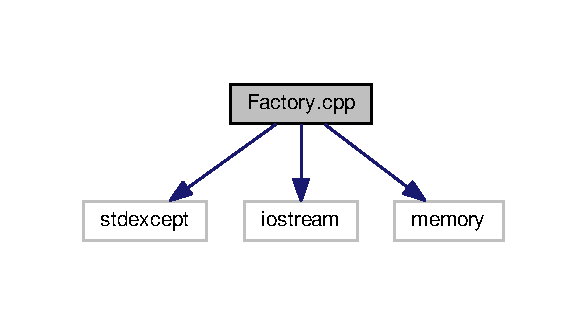
\includegraphics[width=282pt]{Factory_8cpp__incl}
\end{center}
\end{figure}
\subsection*{Classes}
\begin{DoxyCompactItemize}
\item 
class \hyperlink{classPizza}{Pizza}
\item 
class \hyperlink{classHamAndMushroomPizza}{Ham\+And\+Mushroom\+Pizza}
\item 
class \hyperlink{classDeluxePizza}{Deluxe\+Pizza}
\item 
class \hyperlink{classHawaiianPizza}{Hawaiian\+Pizza}
\item 
class \hyperlink{classPizzaFactory}{Pizza\+Factory}
\end{DoxyCompactItemize}
\subsection*{Functions}
\begin{DoxyCompactItemize}
\item 
void \hyperlink{Factory_8cpp_a070ae1b514e4de298f4c34dc2b193ac7}{pizza\+\_\+information} (\hyperlink{classPizzaFactory_a247cf751b7af4fd338a14303c9e67fe4}{Pizza\+Factory\+::\+Pizza\+Type} pizzatype)
\item 
int \hyperlink{Factory_8cpp_ae66f6b31b5ad750f1fe042a706a4e3d4}{main} ()
\end{DoxyCompactItemize}


\subsection{Function Documentation}
\index{Factory.\+cpp@{Factory.\+cpp}!main@{main}}
\index{main@{main}!Factory.\+cpp@{Factory.\+cpp}}
\subsubsection[{\texorpdfstring{main()}{main()}}]{\setlength{\rightskip}{0pt plus 5cm}int main (
\begin{DoxyParamCaption}
{}
\end{DoxyParamCaption}
)}\hypertarget{Factory_8cpp_ae66f6b31b5ad750f1fe042a706a4e3d4}{}\label{Factory_8cpp_ae66f6b31b5ad750f1fe042a706a4e3d4}

\begin{DoxyCode}
58 \{
59     \hyperlink{Factory_8cpp_a070ae1b514e4de298f4c34dc2b193ac7}{pizza\_information}(\hyperlink{classPizzaFactory_a247cf751b7af4fd338a14303c9e67fe4ab47db230a75b01a1a531d9374a57dc23}{PizzaFactory::HamMushroom});
60     \hyperlink{Factory_8cpp_a070ae1b514e4de298f4c34dc2b193ac7}{pizza\_information}(\hyperlink{classPizzaFactory_a247cf751b7af4fd338a14303c9e67fe4ae05ccf2778af31944f7205f550c33e8b}{PizzaFactory::Deluxe});
61     \hyperlink{Factory_8cpp_a070ae1b514e4de298f4c34dc2b193ac7}{pizza\_information}(\hyperlink{classPizzaFactory_a247cf751b7af4fd338a14303c9e67fe4a43552967e3be1afe8d7bf89feb21ba4e}{PizzaFactory::Hawaiian});
62 \}\end{DoxyCode}


Here is the call graph for this function\+:
\nopagebreak
\begin{figure}[H]
\begin{center}
\leavevmode
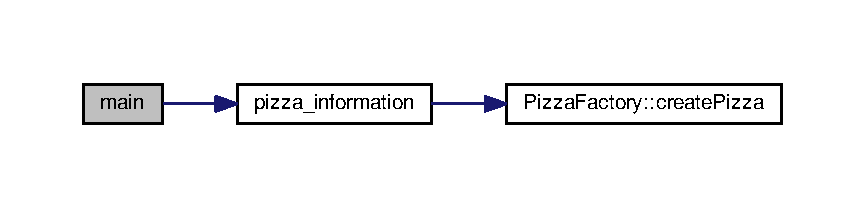
\includegraphics[width=350pt]{Factory_8cpp_ae66f6b31b5ad750f1fe042a706a4e3d4_cgraph}
\end{center}
\end{figure}


\index{Factory.\+cpp@{Factory.\+cpp}!pizza\+\_\+information@{pizza\+\_\+information}}
\index{pizza\+\_\+information@{pizza\+\_\+information}!Factory.\+cpp@{Factory.\+cpp}}
\subsubsection[{\texorpdfstring{pizza\+\_\+information(\+Pizza\+Factory\+::\+Pizza\+Type pizzatype)}{pizza_information(PizzaFactory::PizzaType pizzatype)}}]{\setlength{\rightskip}{0pt plus 5cm}void pizza\+\_\+information (
\begin{DoxyParamCaption}
\item[{{\bf Pizza\+Factory\+::\+Pizza\+Type}}]{pizzatype}
\end{DoxyParamCaption}
)}\hypertarget{Factory_8cpp_a070ae1b514e4de298f4c34dc2b193ac7}{}\label{Factory_8cpp_a070ae1b514e4de298f4c34dc2b193ac7}

\begin{DoxyCode}
52 \{
53     unique\_ptr<Pizza> pizza = \hyperlink{classPizzaFactory_ae03b206abf337720e9f019eb735d6131}{PizzaFactory::createPizza}(pizzatype);
54     cout << \textcolor{stringliteral}{"Price of "} << pizzatype << \textcolor{stringliteral}{" is "} << pizza->getPrice() << std::endl;
55 \}
\end{DoxyCode}


Here is the call graph for this function\+:
\nopagebreak
\begin{figure}[H]
\begin{center}
\leavevmode
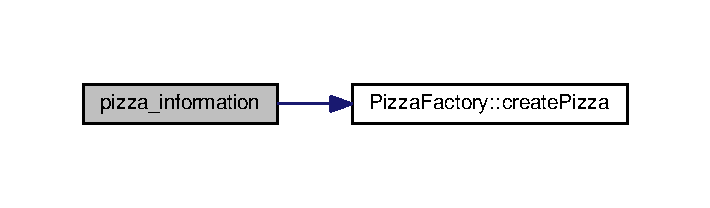
\includegraphics[width=341pt]{Factory_8cpp_a070ae1b514e4de298f4c34dc2b193ac7_cgraph}
\end{center}
\end{figure}



%--- End generated contents ---

% Index
\backmatter
\newpage
\phantomsection
\clearemptydoublepage
\addcontentsline{toc}{chapter}{Index}
\printindex

\end{document}
